% !TEX root = rapport.tex

\section{Future}
There is evidently no way to know with certainty what the future has in store, and this is true also when it comes to technical development. On the other hand, knowing what the prominent factors are, one can more easily predict this development. It can be seen that the history of input and output devices has not had a tight connection to that of computer processing power and memory, although the lack of which can delay the popularisation of such devices. Some examples of this are mentioned above; the computer terminal, which gained in popularity first when computer memory became more easily available and the use of neural networks (not only for sound processing) which gained in popularity again in the 1980's, when processing power had increased. According to the famous Moore's law[reference], the number of transistors and hence chip performance doubles approximately every two years, further leading us to believe that this is not the main issue.

The development rather aspires to ease the interaction either by making devices more portable and available or to remove the obstacles present in the interaction. This is well examplified by the "Google Glass" project currently under development, which aims to provide both higher portability and more natural input methods. Additionally, this section will cover the use of gesture based systems, and systems to control devices directly by thought. 

\subsection{Google Glass}


\subsection{Gesture control}
Gesture control is a means of interaction that uses either hand-gestures or full-body gestures to control and interact with a device. In a way, this form of control aims to immitate human-human interaction by removing the need of physical interaction with any device. Possibly the first such system was the \emph{theremin} developed in 1919/1920 by Leon Theremin. The theremin is an electronic musical instrument, operated by hand gestures. Depending on the position of the hands in relation to the antennas, sounds of different frequencies are generated.

This is an early example of how hand gesture control can be useful and intuitive in certain contexts. There are several contexts where gesture control can be useful. Separating the user from the machine can be useful to protect the physical machine from abuse, as the system is worked from a distance. During a presentation, the speaker could avoid the obstructing act of changing slides by using hand gestures to signal this instead, and if the session is filmed, hand gestures could easily notify the camera to focus on a certain area on a blackboard, screen or object being exhibited. They are often useful in the same settings where voice recognition would be useful, but does not suffer from the disadvantage of being sensitive to noise and does not break the user's flow when communicating.[ref: hardenberg] Tracking mouth movements can also aid in speech recognition, and speech and gesture recognition can also be used in combination.[ref: A SURVEY OF SPEECH-HAND GESTURE RECOGNITION FOR THE DEVELOPMENT OF
MULTIMODAL INTERFACES IN COMPUTER GAMES, Combined Gesture-Speech Analysis and Speech Driven Gesture Synthesis]

There are several difficulties involved with gesture recognition, subject to current study. To be able to recognise gestures the systems are dependent on a camera, which needs be positioned in a way where it can catch the relevant movements of the subject and must also have a rather high resolution and frame frequency in order to cope with the speed of human movement. Furthermore, this must be combined with fast and accurate algorithms to detect and track the movement reliably. Other than the technical issues, there is the issue of ease-of-use. A techique that aims to provide a natural interface such as that of regular human interaction must be quite tolerant - the input must be done on the terms of the user. 

An example of a gesture based system is the \emph{SixthSense} developed at the MIT Media Lab, a mobile gesture based system which additionaly utilises a mini-projector. The camera and the projector hang around the neck of the user similar to a pendant. The camera recognises the users hand-gestures to perform the requests, and can optionally use the projector to project data onto a surface. What is especially interesting with the SixthSense is its user-interface. In a traditional system, the user interacts with a user-interface against the computer whereas the goal of the system is to use the user's normal setting - the physical world. Ideally, the user would interact with objects as usual with the computer aiding when appropriate, see figure [REF FIGURE].


%http://upload.wikimedia.org/wikipedia/en/thumb/a/ab/SixthSense_Augmented_Newspaper.jpg/800px-SixthSense_Augmented_Newspaper.jpg
%http://en.wikipedia.org/wiki/File:SixthSense_Augmented_Newspaper.jpg
\begin{figure}[]
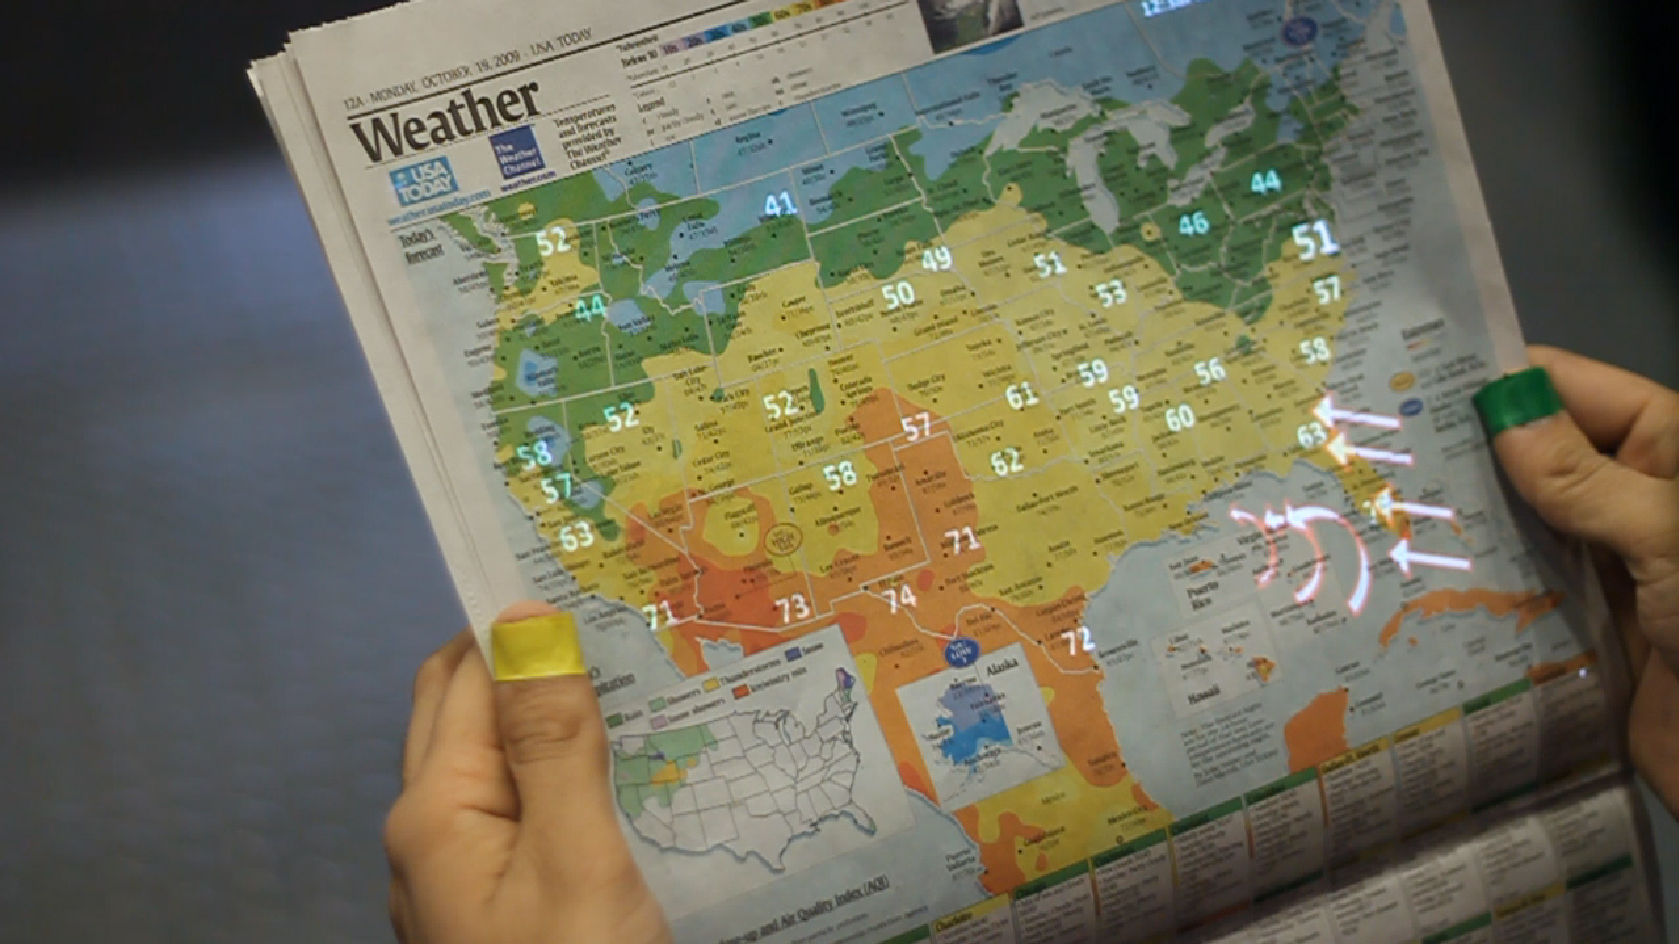
\includegraphics[width=0.8\textwidth] {bilder/newspaper.jpg}
\caption{The SixthSense interacting with a newspaper augmented with weather data.}
\label{sixthsense}
\end{figure}
% Bild på xerox-musen eller mac-musen
\nocite{sixthsense}


\subsection{Brain Computer Interfaces}

Since the early 1990's there has been a lot of research on Brain-Computer Interaction systems. These systems uses brain readings (MRI, EEC, EOpC, \todo{skriv mer specifikt}) techniques to use brain activity as input to a computer. The use of brain-computer interfaces have up to now mostly been used for controlling prostethic devices for persons that have become blind, have lost limbs or lost control of motor functions\todo{ref: 1-s2.0-S0166223606001470-main.pdf **DUBBELKOLLA ATT REF ÄR GILTIG**}, but have in later years also been able to decode pictures from the brain activity \todo{ref: 1-s2.0-S0896627308009586-main.pdf}.

BCI methods can be divided into non-intrusive, partially intrusive and intrusive technologies. Non-intrusive technologies are technologies where the brain activity reading equipment is placed on the outside of the persons head. This requires no surgical procedure and is therefore the easiest and safest method for scanning brain activity. The drawback is that the readings are usually more imprecise than intrusive methods, since the readings are distorted by the skull, however some \todo{ref: pone.0026322.pdf} methods have been developed that give readings comparable to more intrusive approaches.
The partially intrusive methods are methods that require electrodes to be placed inside the persons skull, but outside the grey matter of the brain. This approach removes the distortions caused by the skull, but require surgical procedures that can be dangerous for the patient. The intrusive methods are methods where electrodes are placed into the grey matter of the person. This gives the highest accuracy, down to neuron level, but cause tissue scarring on the person, since the body tries to get rid of the foreign object.

The history of brain activity reading started in 1924 when Hans Berger discovered the electrical activity of the brain and the first EEG equipment was constructed. This equipment enabled the reading of electromagnetic activity in the brain. During the 60's and 70's more research on this area has allowed \todo{personer} X to implant electrodes in the brains of monkeys, which were able to control a robotic arm \todo{ref: Science-1989-Georgopoulos-234-6.pdf}.

%skriv något om hur det har applicerats på människor

%skriv om dagens användningsområden
A main point of interest for brain-computer interfaces during the last year has been for controlling computer games \todo{ref: 10.1007-978-3-642-33542-6\_33.pdf}.

%skriv om potentiella framtida användningar

%skriv om etiska ställningstaganden som krävs.
The use of BCI comes with a number of ethic questions, the most important of which are side-effects from intrusive BC interfaces, mind reading and mind control.
%side-effects
Mind reading could be used for many purposes, some of which are of a very questionable ethical nature. While mind reading can be a help or even the only way to communicate for persons that have lost all motor skills, even the use of the eyes. On the other hand mind reading could interfere with the privacy of that person if the mind reading goes on outside the users will. This could also present a problem in interrogation settings \todo{skriv mer.}.

